\chapter{Introducci\'on}
\label{ch:intro}

La f\'isica de astropart\'iculas experimenta en la actualidad un desarrollo sin precedentes. 
El mensajero tradicional del cielo, el fot\'on, ha sido complementado a principios del siglo XX mediante la observaci\'on de part\'iculas cargadas (rayos c\'osmicos) y, durante las \'ultimas d\'ecadas se han realizado esfuerzos en el desarrollo de la astrof\'isica de neutrinos.
Todos estos mensajeros acarrean informaci\'on sobre la fuente que los produjo, lo que los convierte en nuestra ventana de acceso al cosmos.

El desarrollo de la astronom\'ia de neutrinos lleva varias d\'ecadas de desarrollo. 
El 23 de febrero de 1987 Kamiokande II recibi\'o la se\~nal de 11 neutrinos con energ\'ias en el \'orden del MeV, mientras que simult\'aneamente el detector IBM observ\'o otros 8.
Estos eventos, en coincidencia con la observaci\'on de la supernova SN 1987A, dieron lugar a la primera observaci\'on de neutrinos provenientes de una fuente extra gal\'actica.
Ya en esta d\'ecada, IceCube ha realizando las primeras mediciones de neutrinos c\'osmicos en energ\'ias del PeV~\cite{cite:IceCube1}.
Estos descubrimientos admiten una nueva mirada al universo, expandiendo as\'i las posibilidades de observaci\'on.
Por un lado los rayos c\'osmicos cargados son deflectados debido a los campos magn\'eticos intergal\'acticos mientras que por otro, los fotones son absorbidos en las zonas opacas del espacio. 
Sin embargo, los neutrinos no sufren ninguna de estas alteraciones ya que no poseen carga el\'ectrica y adem\'as, como s\'olo interact\'uan mediante fuerza d\'ebil y su secci\'on efic\'az es peque\~na, no son retenidos en las zonas densas del universo.
Esta cualidad, que les provee muy buenas cualidades a la hora de trasladar informaci\'on de un punto a otro del cosmos, los hace extremadamente dif\'iciles de detectar en al tierra, lo que representa un desaf\'io muy interesante de abordar.
% Existe una gran cantidad de rese\~nas sobre el estado del \'area, como por ejemplo \cite{XXX}, en las que se remarca el potencial de utilizar el neutrino como mensajero c\'osmico.

En esta tesis se trata la detecci\'on de neutrinos c\'osmicos ultra energ\'eticos mediante detectores de superficie, y se divide en dos partes.
En la primera se presenta la medici\'on del flujo difuso a neutrinos en el rango energ\'etico de \cant{10^{17}}{eV} a \cant{10^{20}}{eV} con el detector de superficie del Observatorio Pierre Auger.
El cap\'itulo \ref{ch:easAuger} contiene una introducci\'on a la f\'isica de las lluvias atmosf\'ericas extendidas que generan los rayos c\'osmicos ultra energ\'eticos. 
Luego, en el cap\'itulo \ref{ch:detectorAuger} se realiza un recuento de las caracter\'isticas m\'as importantes del detector de superficie del Observatorio Pierre Auger.
M\'as adelante, en el ca\'itulo \ref{ch:estrategiaAuger} se detalla la estrategia utilizada en el experimento para medir el flujo de neutrinos c\'osmicos ultra energ\'eticos.
El proceso de simulaci\'on de la se\~nal esperada sobre el detector se aborda en el cap\'itulo \ref{ch:simulacionAuger}, mientras que la reconstrucci\'on y selecci\'on de los eventos iniciados por neutrinos se trata en el cap\'itulo \ref{ch:selAuger}.
Por \'ultimo en el cap\'itulo \ref{ch:resAuger} se describe el c\'alculo de la exposici\'on del observatorio al flujo de neutrinos, la b\'usqueda de candidatos y la comparaci\'on de los resultados con las predicciones te\'oricas.

La segunda parte de la tesis se enfoca en estimar el desempe\~no que podr\'ia alcanzar un detector de superficie conformado por 90000 antenas de radio a la hora de medir el flujo de neutrinos c\'osmicos ultra energ\'eticos.
El cap\'itulo \ref{ch:motRadio} se dedica a motivar el estudio de este tipo de detectores.
Mientras que en el cap\'itulo \ref{ch:easRadio}, y como complemento al cap\'itulo \ref{ch:easAuger}, se revisa la emisi\'on de ondas de radio de las lluvias atmosf\'ericas extendidas.
Los m\'etodos empleados en la simulaci\'on de la se\~nal sobre el detector se detallan en el cap\'itulo \ref{ch:simulacionRadio} y su caracterizaci\'on en el cap\'itulo \ref{ch:caracterizacionRadio}.
Finalmente, en el cap\'itulo \ref{ch:resultadosRadio} se aborda tanto la factibilidad de la detecci\'on como el c\'alculo de la exposici\'on en un arreglo de antenas de radio.

\section{Importancia de la detecci\'on de neutrinos c\'osmicos}
%
%
%%
%%%
% 	VER EL PROPOSAL DE GRAND!
%%%
%%
%
%
El estudio de rayos c\'osmicos ultra energ\'eticos (UHECRs por sus siglas en ingl\'es) ha estimulado en gran medida la actividad experimental y te\'orica en el campo de la astrof\'isica.
Aunque su espectro de energ\'ia ha sido caracterizado en un rango sorprendente, que comprende 14 \'ordenes de magnitud, quedan todav\'ia muchos misterios por resolver, como su origen y sus mecanismos de aceleraci\'on.
En esta direcci\'on, la medici\'on de UHECRs cargados presenta dos grandes limitaciones, su deflexi\'on en los campos magn\'eticos existentes en el cosmos y lo que se conoce como el corte GZK.
A energ\'ias por debajo de los \cant{10^{19.5}}{eV} las trayectorias desde la fuente se ven modificadas debido a la interacci\'on con los campos magn\'eticos gal\'acticos e intergal\'acticos lo que implica que la direcci\'on de arribo de los rayos a la tierra no apunta a la fuente.
Por otro lado, el corte GZK refiere al mecanismo propuesto por Greisen, Zatsepin y Kusmin~\cite{cite:Greisen,cite:Zatsepin}, que provoca una caida abrupta en el flujo de UHECRs por encima de \cant{5\times10^{19}}{eV}.
Este efecto se debe a la p\'erdida de energ\'ia inducida por la interacci\'on entre hadrones y el fondo c\'osmico de microondas (CMB por sus siglas en ingl\'es), via la siguiente reacci\'on:
%
\begin{equation}
p + \gamma_{\rm CMB}\, \rightarrow\, \Delta^{+}(1232)  \rightarrow p +\pi^{0}\quad {\rm or}\quad n +\pi^{+}
\end{equation}
%
La longitud de atenuaci\'on para este proceso es $L_{att}=\frac{L_{int}}{y}$, donde $y$ es la fracci\'on de energ\'ia perdida por longitud de interacci\'on y $L_{int}$ es la longitud de interacci\'on, dada por $L_{int}=(\sigma_{p\gamma}\times n_{\gamma})^{-1}$.
Valores t\'ipicos son $\sigma_{p\gamma}\sim 10^{-28}$~cm$^{2}$, $ n_{\gamma}=410\,{\rm cm}^{-3}$ and $y\sim0.5$\footnote{$y\sim0.2$ a la energ\'ia de corte y se incrementa hasta 0.5.}, resultando en 
% \begin{equation}
$L_{att}=(\sigma_{p\gamma}\times n_{\gamma}\times y)^{-1}\sim 15\mbox{ }{\rm Mpc}$. 
Ya que a estas energ\'ias los rayos c\'osmicos son mayormente extra gal\'acticos, el corte GZK limita la m\'axima energ\'ia que puede ser observada en la tierra y provocando una supresi\'on del flujo por encima de los \cant{50}{EeV}.
En la figura \ref{fig:protProp} se muestra la longitud $L_{att}$ como funci\'on de la energ\'ia para protones y n\'ucleos de hierro. 
Es posible observar como a partir de los \cant{50}{EeV} esta cantidad decae hasta un tama\~no inferior al del Super cluster de Virgo, a los \cant{1000}{EeV}.
%
\begin{figure}[ht]
	\begin{center}
	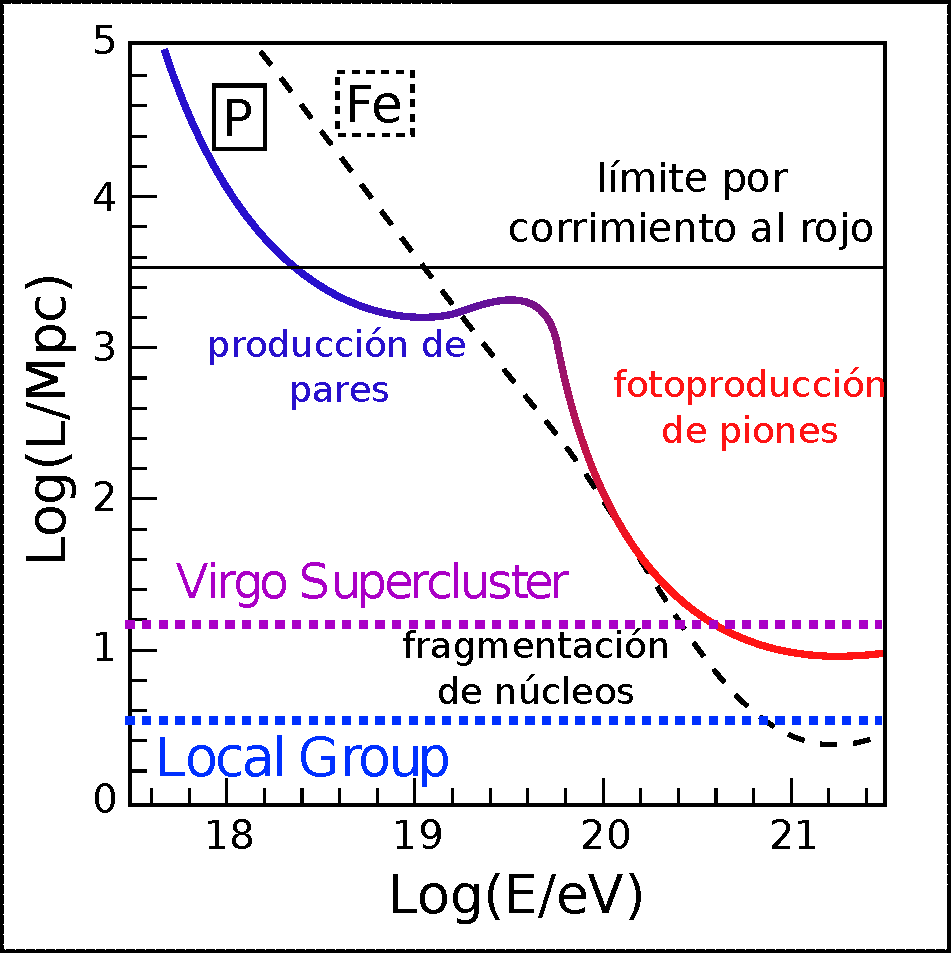
\includegraphics[width=0.55\textwidth]{fig/introduccion/proton_propaga_espanol}
	\caption{\label{fig:protProp} Longitud de atenuaci\'on como funci\'on de la energ\'ia para protones y n\'ucleos de hierro. Se observa que a partir de \cant{50}{EeV} ($\log{E/eV}=18$) esta cantidad decae hasta el tama\~no del Super cluster de Virgo a los \cant{1000}{EeV}.}
	\end{center}
\end{figure}
%

Por otro lado, el observatorio Pierre Auger ha medido el flujo de rayos c\'osmicos combinando un detector de superficie con t\'ecnicas de fluorescencia y ha acumulado suficiente estad\'istica para medir el flujo con presici\'on hasta alrededor de \cant{2\times10^{20}}{eV}. 
Tambi\'en pudo corroborar que la supresi\'on del flujo sucede a energ\'ias superiores a los \cant{10^{19.6}}{eV}~\cite{cite:AugerSpectrum}, tal como se observa en la figura \ref{fig:specGZK}.
%
\begin{figure}[ht]
	\begin{center}
	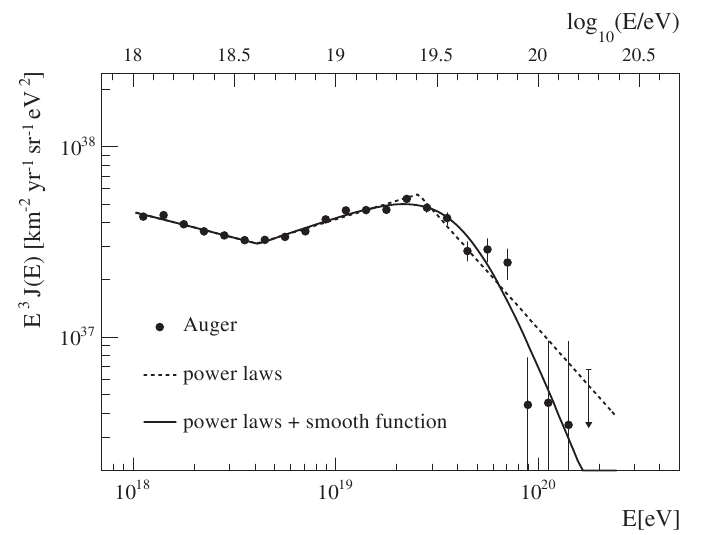
\includegraphics[width=\textwidth]{fig/introduccion/spectrum_withGZK}
	\caption{\label{fig:specGZK} Espectro de UHECRs medido con el observatorio Pierre Auger. En l\'inea punteada se muestra el ajuste por leyes de potencia partidas y en l\'inea llena la dos leyes de potencia y una funci\'on suave. Las barras corresponden al error estad\'istico de cada punto, mientras que el error sistem\'atico representa el $22\%$ de la energ\'ia.}
	\end{center}
\end{figure}

De manera similar, el flujo de fotones ultra energ\'eticos, por encima de \cant{\sim 10^{14}}{eV}, no puede ser de naturaleza extra gal\'actica, debido a la producci\'on de pares en la interacci\'on con fotones del fondo de microondas, seg\'un\cite{cite:photonInt1,cite:photonInt2}:
%
\begin{equation}
\gamma_{UHE} + \gamma_{CMB} \rightarrow e^- + e^+
\end{equation}
%
En la figura \ref{fig:photProp} se grfica la longitud de atenuaci\'on de los fotones como funci\'on de la energ\'ia\footnote{La longitud de atenuaci\'on corresponde a la distancia necesaria para que el flujo decaiga a la mitad.}
%
\begin{figure}[ht]
	\begin{center}
	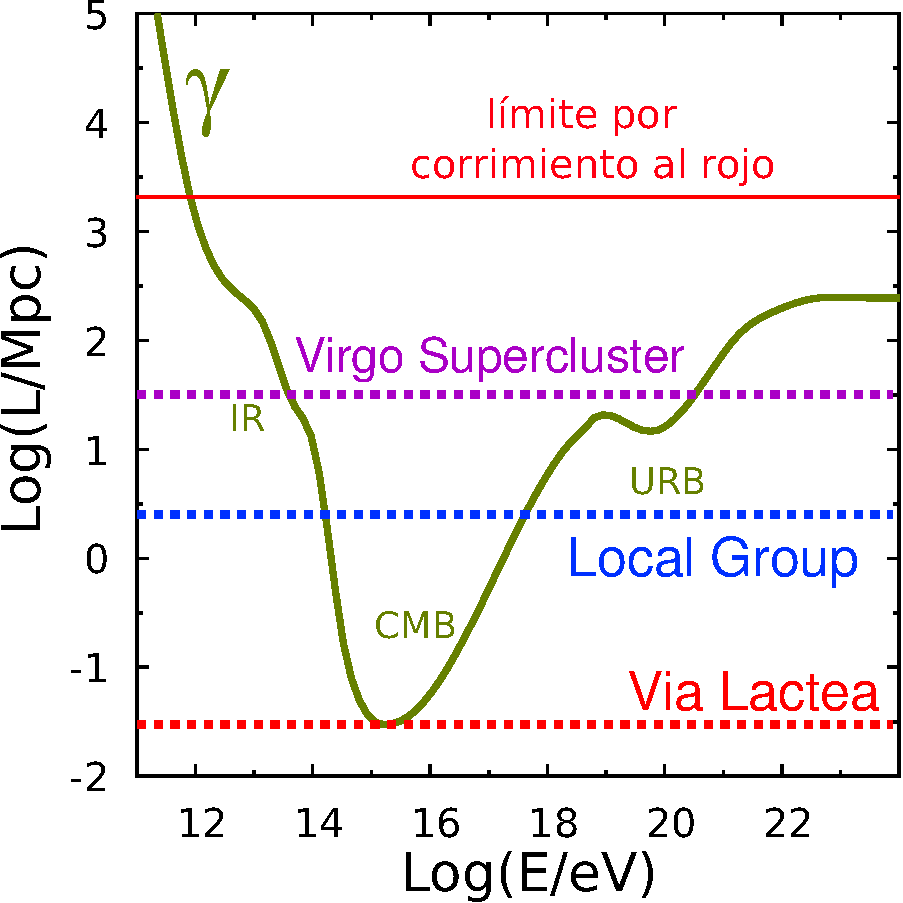
\includegraphics[width=0.55\textwidth]{fig/introduccion/photon_propaga_espanol}
	\caption{\label{fig:photProp} Longitud de atenuaci\'on para fotones. Los $\gamma$ con energ\'ias entre \cant{10^{14}}{eV} y \cant{10^{18}}{eV} pr\'acticamente no pueden alcanzar la tierra desde distancias mayores a \cant{1}{Mpc}. Las etiquetas IR, CMB y URB (ver texto) corresponden al fondo dominante contra el que interact\'uan los $\gamma_{UHE}$.}
	\end{center}
\end{figure}
%
Dependiendo de la energ\'ia, los $\gamma_{UHE}$ pueden interactuar tambi\'en con el fondo de radiaci\'on infraroja (IR)\cite{cite:IR} y con el fondo de radio universal (URB)\cite{cite:URB}.

Como consecuencia el tercer mensajero $-$ el neutrino $-$ cobra una importancia adicional, lo que convirti\'o su detecci\'on en uno de los mayores logros de la astrof\'isica contempor\'anea.
Esto se debe a que los neutrinos no sufren ninguna de las desventajas mencionadas hasta el momento. 
Debido a que interact\'uan mediante interacci\'on d\'ebil y a que su secci\'on efic\'az resulta extremadamente peque\~na, pueden viajar distancias cosmol\'ogicas e incluso escapar de la regi\'on en la que fueron producidos casi sin p\'erdidas de energ\'ia.
Por otro lado, debido a que son el\'ectricamente neutros su trayectoria no se ver\'a deflectada debido a la interacci\'on con los campos magn\'eticos intra y extra gal\'acticos.
Por este motivo, la direcci\'on de arribo de los neutrinos c\'osmicos detectados guardar\'a completamente la informaci\'on del lugar del universo en el que fueron producidos.
Por estos motivos, representan una opci\'on \'unica que permite detectar directamente posibles fuentes de UHECRs.

En las siguientes secciones de este cap\'itulo se presentar\'a una discusi\'on sobre las posibles fuentes y flujos de neutrinos c\'osmicos ultra energ\'eticos, a saber, el mecanismo GZK, n\'ucleos de galaxias activos (AGN) y explosiones de rayos gamma (GRB).
Tambi\'en se realizar\'a un recuento de los ezfuersos experimentales pasados, presentes y futuros en este campo.

\section{Posibles fuentes y flujos esperados}

Existen varios modelos en la literatura que predicen flujos de neutrinos c\'osmicos ultra energ\'eticos.
La la supresi\'on observada en el flujo por encima de los \cant{50}{EeV} refuerza la idea de la existencia de un flujo difuso de neutrinos cosmog\'enicos.
En este caso, estos son producidos durante la propagaci\'on de un UHECR a trav\'es del universo. 
Adem\'as pueden ser producidos en la aceleraci\'on de protones y n\'ucleos en n\'ucleos de galaxias activos (o AGN por sus siglas en ingl\'es)\cite{cite:nuAGN} o por producci\'on de fotopiones en explosiones de rayos gamma (GRB por sus siglas en ingles)\cite{cite:nuGRB}.
% Detectores como AMANDA o IceCube, su sucesor, se encuentran bien posicionados para realizar b\'usquedas de fuentes con espectros de ley de potencia fuertes ($\propto E^{-2}$) en el rango que comprende desde el TeV  hasta el PeV. 
% Para fuentes cuyo flujo presenta un m\'aximo en energ\'ias por encima de los \cant{100}{PeV} el flujo predicho resulta ser peque\~no, requiriendo detectores con mayor exposici\'on.

% Otros posibles mecanismos de producci\'on de neutrinos c\'osmicos estan relacionados con el decaimiento de part\'iculas ex\'oticas extremadamente masivas tales como defectos topol\'ogicos\cite{cite:nuTopDefects}, o con la interacci\'on de neutrinos energ\'eticos con el fondo de neutrinos del Big-Bang via la resonancia Z-burst\cite{cite:nuZBurst_init}.
% Estos flujos, que pretend\'ian explicar el origen de los rayos c\'osmicos ultra energ\'eticos, han sido fuertemente constre\~nidos por los experimentos m\'as recientes\cite{cite:nuConstraintsTD}.
% En las siguientes secciones se desarrollas las ideas enumeradas hasta aqu\'i.

	\subsection{Neutrinos GZK}
	\label{sbsc:introGZK}
	Greisen, Zatsepin and Kusmin propusieron que los rayos c\'osmicos cuya energ\'ia supere los \cant{5\times10^{19}}{eV}, al propagarse por el universo interactuar\'an con el fondo de microondas produciendo neutrinos, seg\'un la ecuaci\'on \ref{eq:pionDecay}.
	\begin{equation}\label{eq:pionDecay}
	\pi^{+} \rightarrow \mu^{+}+ \nu_{\mu} \rightarrow e^{+} + \nu_{e} + \bar{\nu}_{\mu} + \nu_{\mu}
	\end{equation}
	
	La precencia del corte GZK, indica que los UHECRs provienen de fuentes extra gal'acticas.
	Esto implica que los llamados neutrinos GZK son el flujo m'as verosimil entre todas las posibles teor'ias. 
	Sin embargo, su c'alculo contiene una gr\'an cantidad de supuestos que se traducen en incertezas en el resultado final.
	Los factores m\'as relevantes en su determinaci\'on son los siguientes~\cite{cite:nuEngel,cite:nuAve,cite:nuAhlers1,cite:nuAllard1,cite:nuYuksel}:
	
	\textbf{Composici\'on de los UHECRs}: las primeras predicciones sobre el flujo de neutrinos cosmol\'ogicos asum\'ian que los primarios son protones, mientras que recientemente han aparecido resultados en los que se consideran como primarios $^{56}{\rm Fe}$, $^{4}{\rm H}$, $^{16}{\rm O}$ o mezclas entre ellos y con protones\cite{cite:nuAve,cite:nuHooper}.
	Los n\'ucleos m\'as pesados pierden energ\'ia por foto-desintegraci\'on, produciendo n\'ucleos secundarios, que luego producen fotopiones que al decaer generan neutrinos UHE$\nu$.
	Adem\'as, fujos de antineutrinos electr\'onicos son predichos via decaimiento de neutrones\cite{cite:nuFeComposition}, pero su energ\'ia resulta peque\~na para ser detectados por Auger.
	Por otro lado, los flujos que provienen de una composici\'on primaria no pura son peque\~nos cuando se los compara con una composici\'on de protones pura\cite{cite:nuHooper}.
	En particular, la energ\'ia por nucle\'on luego de una fotodesintegraci\'on resulta mucho m\'as peque\~na que la del primario, lo que desfavorece la generaci\'on de neutrinos GZK a trav\'es de este proceso.
	Tambi\'en existen modelos en los que se propone una distribuci\'on de primarios en acuerdo con la composici\'on observada en los rayos c\'osmicos gal\'acticos\cite{cite:nuAllard1}.
	Como consecuencia de estas suposiciones los flujos predichos pueden fluctuar en un \'orden de magnitud.
	 
	Resultados recientes de Auger indican, aunque con cierto nivel de debate, que el flujo de UHECRs se encuentra dominado por n\'ucleos pesados\cite{cite:augerComposition}.
	Sin embargo, mediciones en HiRes y Telescope Array\cite{cite:taComposition} han observado lo opuesto.
	Si se llegase a dar una observaci\'on por encima de las predicciones para primarios pesados, se podr\'ia echar luz sobre este asunto.
	 
	\textbf{Perfil de energ\'ia}: el espectro energ\'etico de los rayos c\'osmicos en el punto de inyecci\'on se supone t\'ipicamente una ley de potencia con la siguiente dependencia en energ\'ia:
	%
	\begin{equation}
		\frac{dN}{dE}=P_{0} \times E^{-\alpha} \times \exp{(-\frac{E}{E_{c}})}
	\end{equation}
	%
	donde $P_0$ es una normalizaci\'on y el \'indice espectral $\alpha$ toma valores entre 1.8 y 2.7, siendo $\alpha\sim2.3$ el m\'as favorecido.
	El corte de energ\'ia en la inyecci\'on, $E_c$ es considerado entre \cant{10^{20}}{eV} y \cant{10^{23}}{eV}.
	Tanto $\alpha$ como $E_c$ dependen de las caracter\'isticas de la fuente y del mecanismo de aceleraci\'on de los rayos c\'osmicos.
	Una vez que estos valores son elegidos, la normalizaci\'on $P_0$ se utiliza para hacer coincidir el flujo con el observado experimentalmente en la Tierra.
	Valores grandes de $\alpha$ o peque\~nos de $E_c$ producen flujos de neutrinos m\'as peque\~nos a energ\'ias de observaci\'on de Auger debido a la disminuci\'on en la cantidad de protones de altas energ\'ia en la fuente.
	
	\textbf{Modelo cosmol\'ogico}: la cosmolog\'ia del universo es otro factor que genera incerteza en la magnitud del flujo de neutrinos GZK. 
	En la actualidad, observaciones astrof\'isicas apuntan hacia modelos con una constante cosmol\'ogica $\Lambda$\cite{cite:Lambda}, en contraste con los c\'alculos de mediados de la d\'ecada del 90, que supon\'ian un universo de Einstein-de Sitter ($\Omega_{M}=1$). 
	El modelo favorecido actualmente posee $\Omega_{\Lambda}=0.7$ y $\Omega_{M}=0.3$\cite{cite:LambdaM}, lo que significa que la energ\'ia oscura representa alrededor del 70\% de la energ\'ia del universo.
	Como consecuencia el universo debi\'o haberse estado expandiendo mas lentamente en el momento en el que los flujos cosmol\'ogicos se generaron, ocasionando un incremento en los flujos esperados para corrimientos al rojo grandes.
	Engel et al. \cite{cite:nuEngel} compararon el flujo derivado de los dos modelos cosmol\'ogicos y encontraron que valores de $\Omega_{\Lambda}=0.7$ podr\'ian ocasionar hasta un 60\% de incremento en el flujo de neutrinos esperado.
	
	\textbf{Evoluci\'on cosmol\'ogica}: la predicci\'on de los flujos de neutrinos dependen fuertemente de la evoluci\'on cosmol\'ogica de de las fuentes de rayos c\'osmicos.
	Existen al menos 4 modelos de evoluci\'on utilizados comunmente en la bibliograf\'ia:
	\begin{enumerate}
	 \item Sin evoluci\'on;
	 \item Star Formation Rate;
	 \item Active Galactic Nuclei-FRII (FRII) y
	 \item Strong Gamma Ray Burst (GRB).
	\end{enumerate}
	
	Las diferencias inducidas por esta elecci\'on puede modificar el flujo esperado en un \'orden de magnitud.
	
	\textbf{Secci\'on efic\'az proton-fot\'on}: el ritmo de producci\'on de neutrinos mediante la interacci\'on:
	%
	\begin{displaymath}
	p + \gamma_{\rm CMB}\, \rightarrow\, \Delta^{+}  \rightarrow p +\pi^{0}\quad {\rm or}\quad n +\pi^{+}
	\end{displaymath}
	%
	viene dado por la secci\'on efic\'az prot\'on-fot\'on, $\sigma_{p\gamma}$.
	Las mediciones de esta cantidad provienen de aceleradores, por lo que se encuentran bien caracterizadas en un rango de energ\'ias totalmente distinto al que corresponde da lugar a la producci\'on de neutrinos.
	
	\textbf{Oscilaciones de neutrinos}: en el decaimiento de un pi\'on, la relaci\'on con la que se producen neutrinos mu\'onicos y electr\'onicos es $2:1$. 
% 	En este trabajo, al menos que se especifique lo contrario, hablar de neutrinos de cierto sabor $\nu_x$, har\'a referencia al par $\nu_x + \bar\nu_x$.
	Dado que los neutrinos oscilan, al recorrer distancias cosmol\'ogicas la relaci\'on entre los flujos $\nu_e :\nu_\mu :\nu_\tau$ de $1:2:0$ en la fuente se transformar\'a en una relaci\'on $1:1:1$ en la tierra.

	%
	Aunque la existencia de los neutrinos cosmog\'enicos es verosimil, los flujos predichos por este mecanismo var\'ian cuatro \'ordenes de magnitud.
	Algunas de estas predicciones se muestran en la figura \ref{fig:flujosGZK} para los tres sabores de neutrinos.
	
	\begin{figure}[ht]
		\begin{center}
		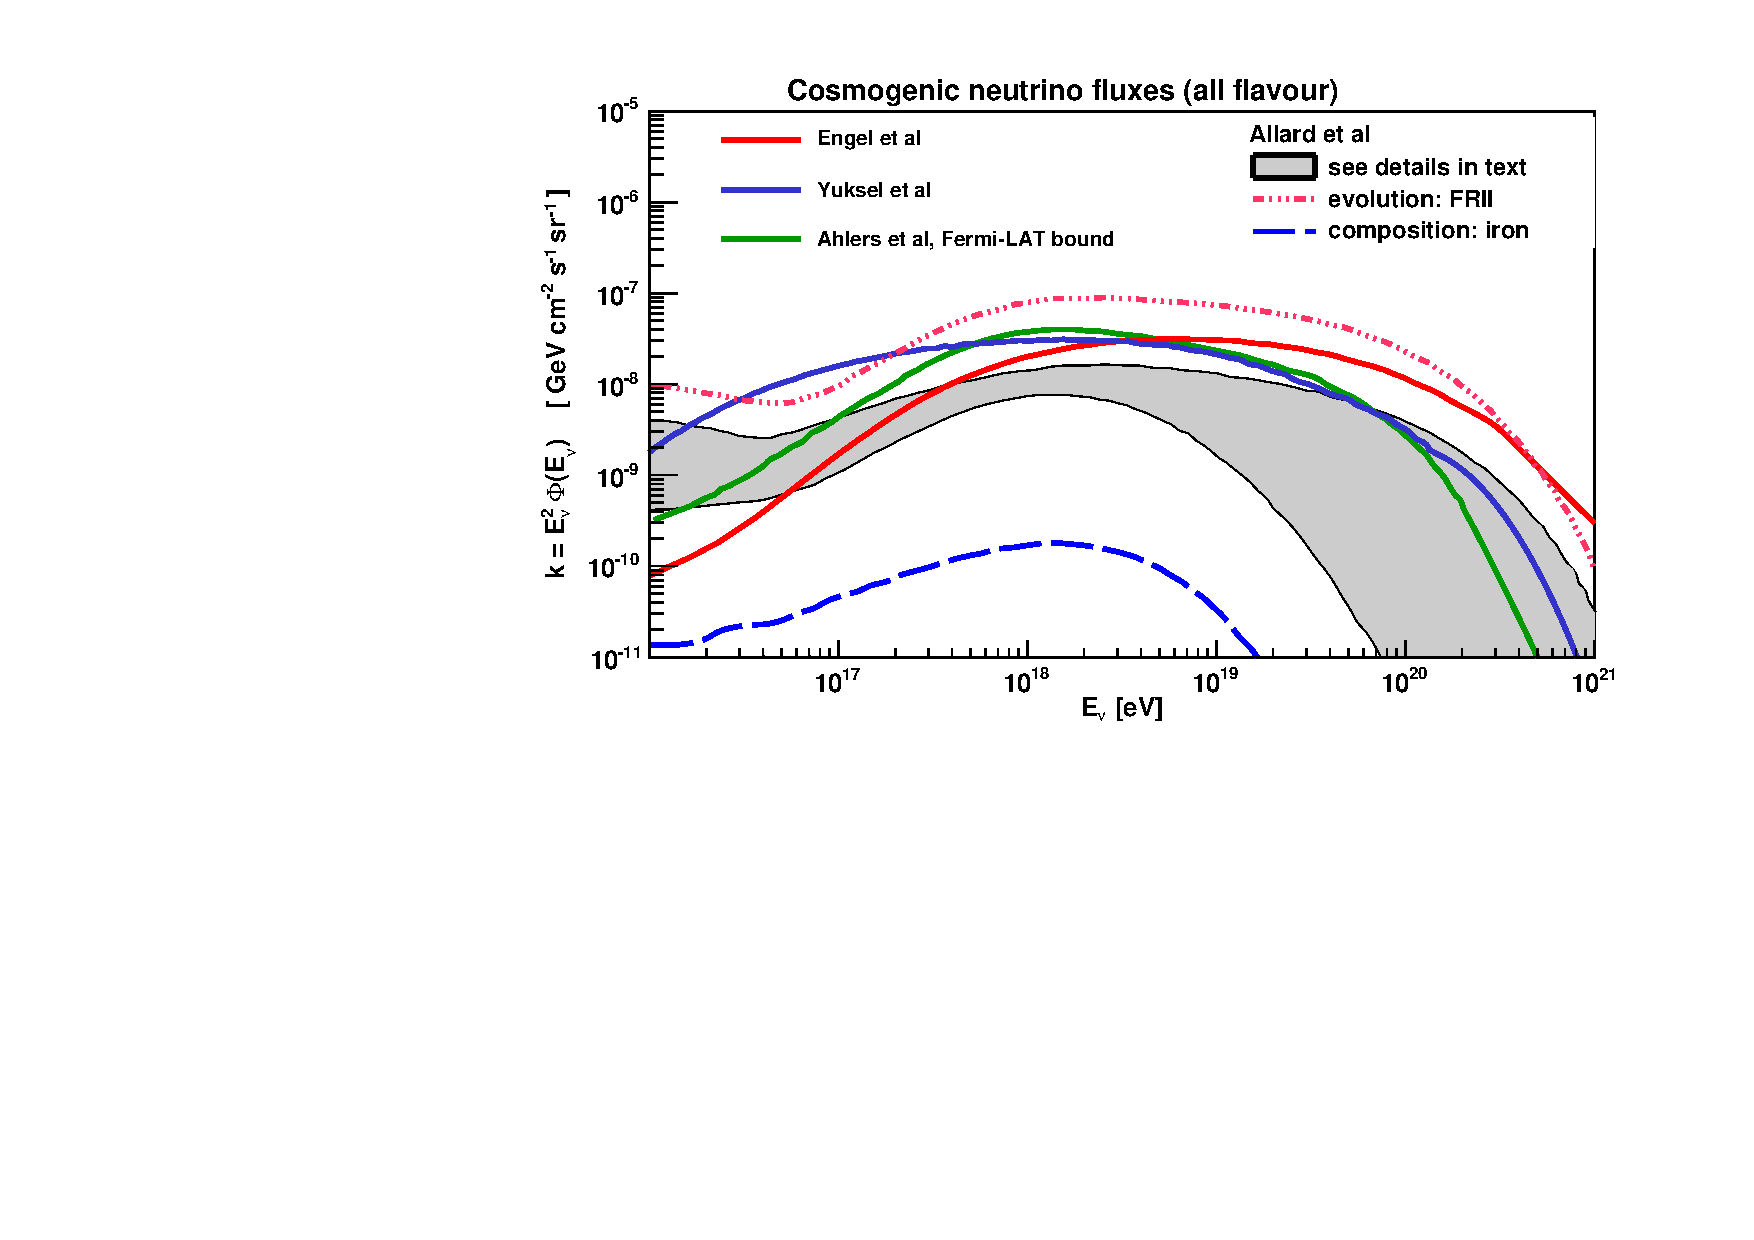
\includegraphics[width=\textwidth]{fig/introduccion/gzk_fluxes}
		\caption{\label{fig:flujosGZK} Flujos cosmog\'enicos para los tres sabores de neutrinos. En todos los casos el modelo cosmol\'ogico usado corresponde con $\Omega_{\Lambda}=0.7$ y $\Omega_{M}=0.3$. 
		En rojo se muestra un flujo GZK t\'ipico para una composici\'on pura de protones, un \'indice $\alpha$ = 2 y \cant{E_{c}=10^{21.5}}{eV}\cite{cite:nuEngel}.
% 		En linea azul s\'olida
% In solid light blue the GRB model for the cosmological evoultion is used\cite{cite:nuYuksel}.
% % In solid green Ref.\cite{cite:nuAhlers1} where they make a prediction using also the measurements of the Fermi-LAT experiment.
% In solid green a prediction using the measurements of the Fermi-LAT experiment\cite{cite:nuAhlers1}.
% The shaded area is obtained from Ref.\cite{cite:nuAllard1}, bracketing a wide range a parameters: 
% several source evolution models (not including uniform and FRII), 
% for pure protons and a mixed Galactic composition. 
% Including the uniform source evolution would lower the prediction by almost an order of magnitude.
% The pink dot-dashed line corresponds to an optimistic scenario with a FRII strong source evolution case with a pure proton composition, 
% % dip transition model 
% and $E_{c}=10^{21.5}$~eV\cite{cite:nuAllard1}. 
% The blue dashed lineis an extreme pessimistic scenario with pure
% iron composition and uniform evolution\cite{cite:nuAllard1}.
% % $E_{c}$ = 1021.5 eV. For the cosmological evolution of the cosmic ray sources, ${\cal H}$(z), they use the
% % aforementioned QSO model with the parameterization of Ref. [33], as given in Eqn.1.7. The
% % default cosmological assumption used is the model with
% 		
		}
		\end{center}
	\end{figure}
	
	\subsection{AGNs y GRBs}
	Los n\'ucleos de galaxias activos (AGN) pueblan de manera isotr\'opica el cielo y representan algunos de los obj\'etos m\'as luminosos en el espacio, con emisiones en el \'orden de los \cant{10^{45\pm3}}{erg/s}\cite{cite:GHZ}.
	Por este motivo no s\'olo son considerados unos de los m\'as fiables candidatos a fuentes de UHECRs, sino que varios autores predicen flujos medibles de neutrinos si la regi\'on de aceleraci\'on se encuentra rodeada de la suficiente cantidad de materia.
	
	Se cree que la enorme radiaci\'on emitida por los AGNs se alimenta de la energ\'ia gravitacional liberada por la materia que cae hacia su centro, en el que se ubica un agujero negro super masivo.
	Durante este proceso, el momento angular provoca que parte del material forme un disco de acresi\'on mientras que otra parte se vea despedida hacia chorros perpendiculares al mismo.
	En tal proceso, los shocks turbulentos aceleran part\'iculas hacia altas energ\'ias.
	De esta manera, una parte significativa de la energ\'ia gravitatoria es transferida a part\'iculas ultra relativistas, via el mecanismo de fermi de primer orden\cite{cite:Fermi1}.
	Por otro lado, la fricci\'on convierte la materia en caida en plasma, que produce un fuerte campo magn\'etico.
	Las colisiones entre los protones ultra relativistas que el intenso campo de fotones del AGN produce neutrinos de alta energ\'ia mediante $p\gamma \rightarrow \pi^{+} + n$ y el subsecuente decaimiento $\pi^{+} \rightarrow \mu^{+} + \nu_{\mu}$ deguido de $\mu^{+} \rightarrow e^{+} + \nu_{e} + \bar{\nu_{\mu}}$.
	
	Otros modelos proponen que los protones colisionan con part\'iculas de gas y polvo, prvocando $pp\,\rightarrow\,\pi s + X$.
	Como en el mecanismo GZK, los neutrinos incluidos inicialmente son $\nu_\mu$ y $\nu_e$ pero las oscilaciones homogeneizan los flujos entre sabores al llegar a la tierra.
	
	Dependiendo del lugar en el que la producci\'on de neutrinos se leva a cabo, existen dos tipos de modelos de producci\'on en AGNs: AGN core y AGN jet.
	En el primer caso, propuesto inicialmente por Stecker et. al.\cite{cite:nuAGN}, los protones acelerados interact\'uan con el campo de fotones dentro del n\'ucleo del AGN. 
	En el segundo modelo, dos jets relativistas emitidos perpendicularmente al disco de acresi\'on formando l\'obulos. 
	Los protones son acelerados mediante el mecanismo de fermi para luego interactuar con fotones del jet y producir neutrinos.
	Su flujo puede ser estimado midiendo la luminosidad para diferentes corrimientos al rojo, como en \cite{cite:Protheroe1}. Por otra parte, Mannheim et al. \cite{cite:Mannheim1}, calcularon el m\'aximo flujo posible proveniente de AGNs a partir de funciones de evoluci\'on de fuentes para blazares, un tipo de AGNs.
	
	Las explosiones de rayos gamma (GRBs) son flashes de fotones $\gamma$ emitidos por fuentes puntuales.
	Estas, representas unas de las explosiones mas fuertes del universo y una posible fuente de neutrinos c\'osmicos ultra energ\'eticos.
	Su emisi\'on ha sido calculada en varias condiciones:
	%
	\begin{enumerate}
	 \item En los modelos de tipo \emph{bola de fuego} o GRB fireball~\cite{cite:grb_Waxman1,cite:grb_Waxman2} la emisi\'on de fotones se produce como producto de colisiones de plasma que se mueve de manera relativista dentro de un chorros de materia (la bola de fuego).
	 Posteriormente el material expulsado colisiona con el medio material externo (por ejemplo el medio interestelar), produciendo radiaci\'on en en un ancho de banda amplio, que comprende desde los rayos X y ultra violetas hasta el visible, conocido como el GRB afterglow.
	 Por otro lado, los electrones y protones acelerados en el jet producen la erupci\'on de fotones de alta energ\'ia mediante radiaci\'on de sincrotr\'on y efecto Compton inverso.
	 Estos fotones de alta energ\'ia interact\'uan con los del afterglow y protones o neutrones del jet produciendo neutrinos ultra energ\'eticos via producci\'on de fotopiones.
	 \item Otro modelo de GRB bastante difundido consiste en los llamados ``modelos de supernova''~\cite{cite:grb_Supernova}. 
	 En estos, protones de la cascara remanente de las supernovas, expulsadas antes del GRB, interact\'uan con los fotones emitidos durante el mismo generando neutrinos ultra energ\'eticos, nuevamente via producci\'on de fotopiones.
	\end{enumerate}
	%
	En la figura \ref{fig:flujosAGN} se muestran los flujos esperados para algunos modelos de AGN y GRB.
	\begin{figure}[ht]
		\begin{center}
		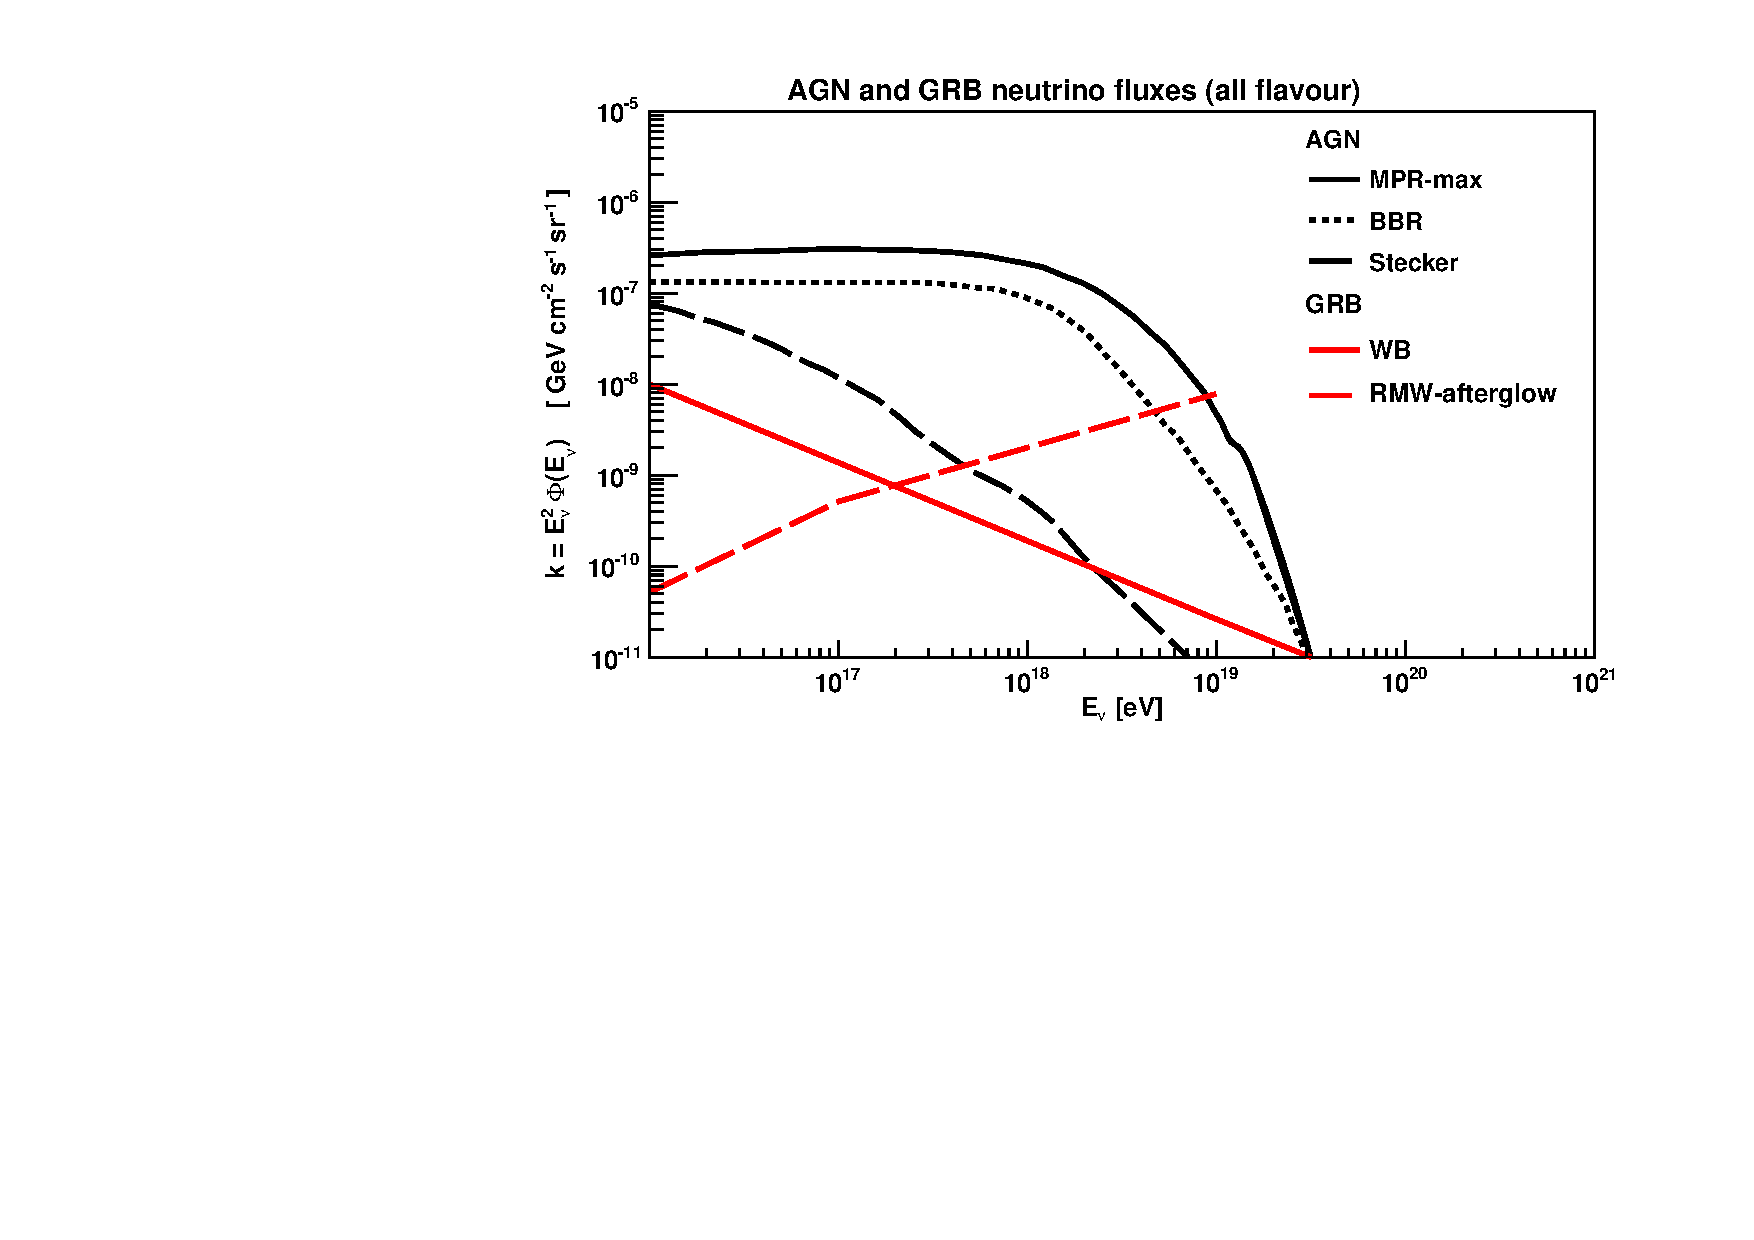
\includegraphics[width=0.75\textwidth]{fig/introduccion/AGN_GRB_nufluxes}
		\caption{\label{fig:flujosAGN} Flujos predichos para AGNs y GRBs. En negro se muestran tres modelos de AGNs\cite{cite:Mannheim1,cite:BBR,cite:SteckerAGN}, mientras que en rojo dos para GRBs\cite{cite:grb_Waxman2,cite:grb_Supernova}.}
		\end{center}
	\end{figure}
	
	\subsection{L\'imite te\'orico al flujo de neutrinos}
	
	E. Waxman y J Bachall establecieron en \cite{cite:WaxmanBahcall1} l\'imites te\'oricos al flujo de neutrinos generados via producci\'on de fotopiones.
	Para ello, consideraron un espectro en las fuentes de la forma $dN_{CR}/dE_{CR}\propto E_{CR}^{-2}$, consistente con el producido mediante el mecanismo de aceleraci\'on de Fermi~\cite{cite:Waxman1}.
	Bajo el supuesto de que la fracci\'on de energ\'ia que se transmite al mes\'on en la producci\'on es independiente de la energ\'ia del primario, el espectro de neutrinos resultante en el decaimiento subsiguiente tambien sigue una ley de potencia $\propto E^{-2}$.
	Asumiento que toda la energ\'ia acarreada por los protones es transmitida a piones en colisiones p-p, el flujo de neutrinos asociado no puede exceder el de los primarios.
	De esta manera lo autores llegaron a una cota superior al flujo utilizando un modelo de no evoluci\'on con el redshift y el modelo cosmol\'ogico \emph{Quasi Stellar Objects}.
	Cabe destacar que en la bibliograf\'ia no existe una cota inferior al flujo de neutrinos ultra energ\'eticos.
	
% 	\subsection{Fuentes no convencionales}
% 	
% 	Este tipo de modelos fueron ropuestos para 
% 	
% 	
% 	\begin{figure}[ht]
% 		\begin{center}
% 		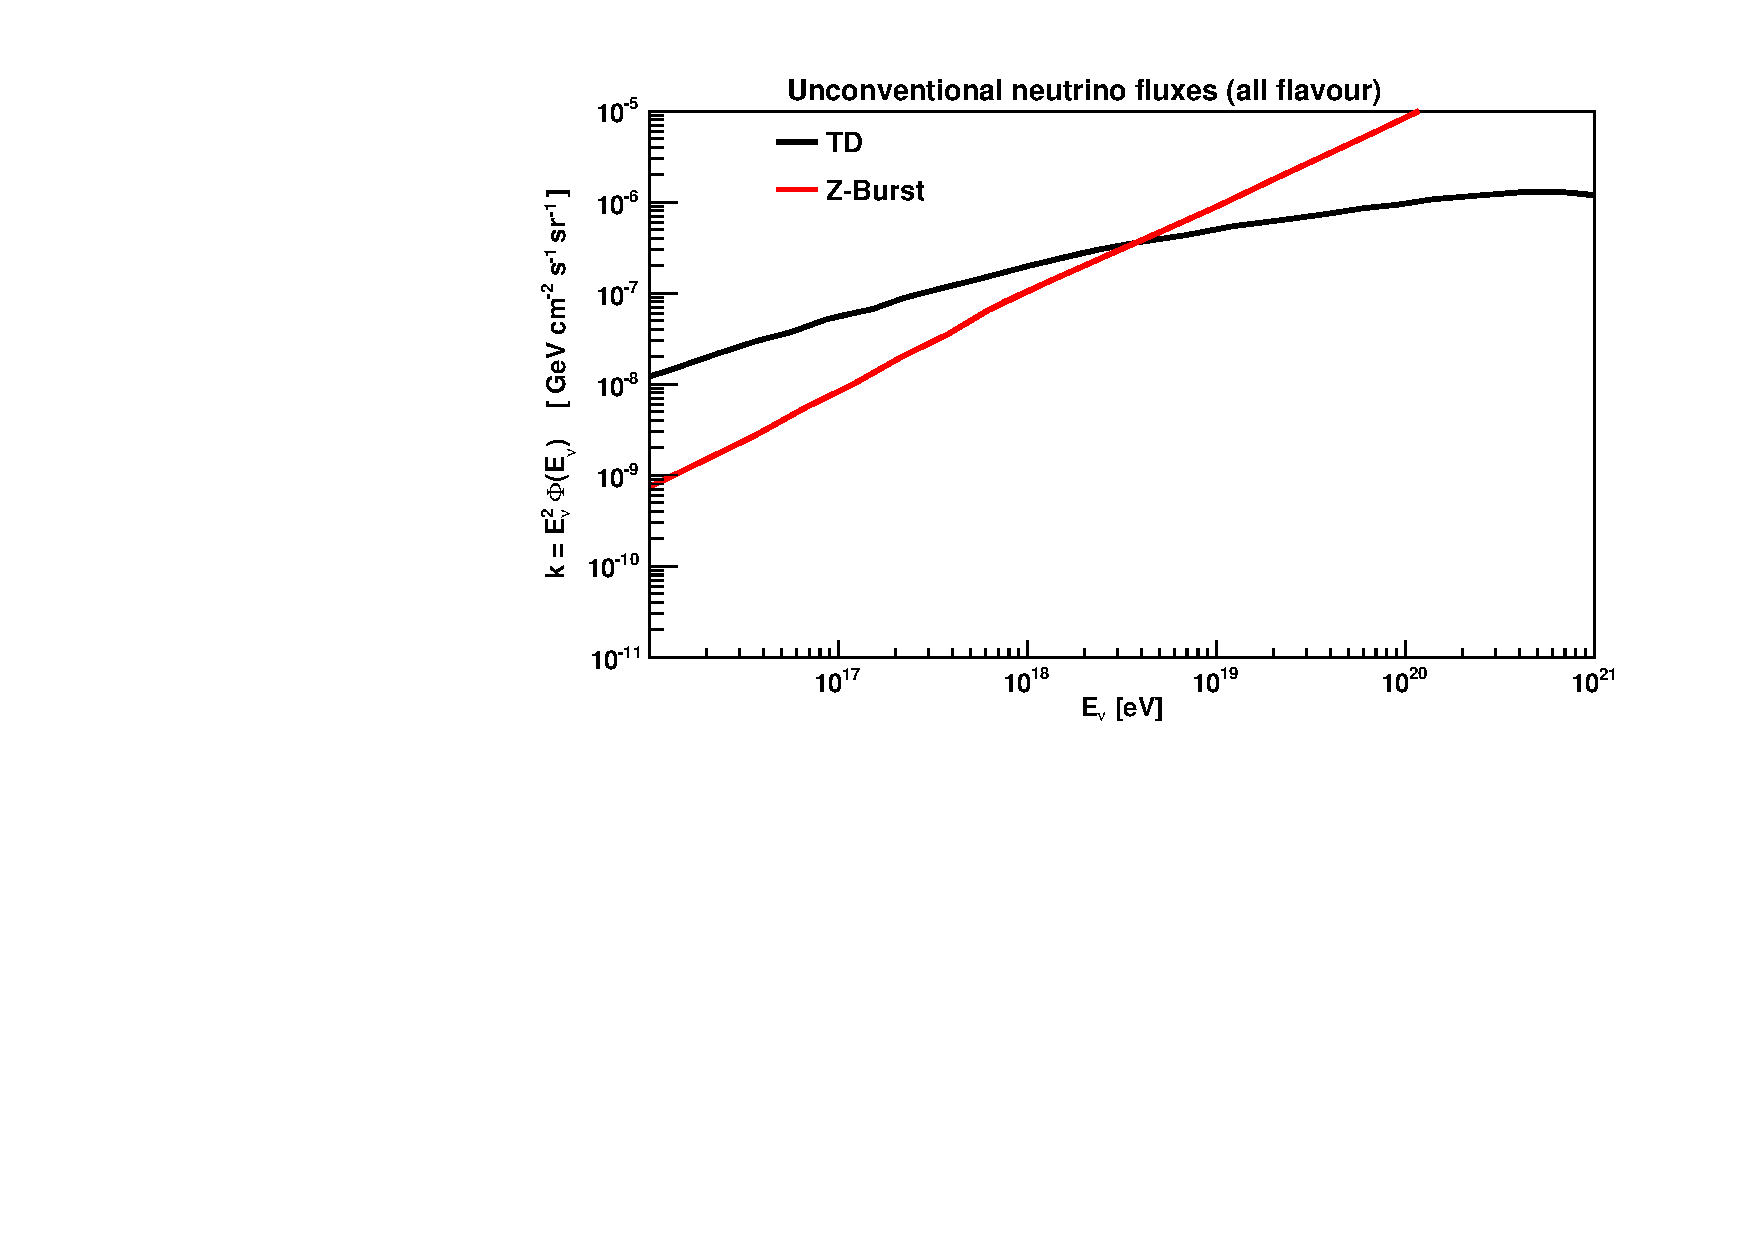
\includegraphics[width=0.75\textwidth]{fig/introduccion/unconventional_nuFluxes}
% 		\caption{\label{fig:flujosNoConv} }
% 		\end{center}
% 	\end{figure}

\section{Búsquedas de neutrinos cósmicos ultra energéticos}

En la actualidad existen diversos experimentos que desarrollan b\'usquedas de neutrinos c\'osmicos ultraenerg\'eticos. 
En \cite{cite:nuSearchReview1} puede encontrarse un recuento extensivo de los mismos as\'i como el estado de su detecci\'on. 
En todos los casos se utiliza un blanco masivo con el que interact\'uan los neutrinos incidentes y se busca medir los efectos de tal interacci\'on.
En particular, en los distintos experimentos el blanco puede consistir en agua, hielo, el aire de la atm\'osfera terrestre, la corteza terrestre o incluso grandes dep\'ositos naturales de sal.
En cuanto a la detecci\'on propiamente dicha, en la actualidad existen varias t\'ecnicas implementadas, que comprenden entre otras, detectores \'opticos, de radio y de part\'iculas.

	\subsection{Detectores \'opticos}
	Las part\'iculas generadas en la interacci\'on entre neutrinos ultra energ\'eticos y medios densos viajan usualmente a velocidades superiores a las de la luz en dicho medio.
	Por ende, si el medio es transparente la luz \cher{} generada en este proceso puede ser capturada mediante fotomultiplicadores.
	
	A finales de los 90's el experimento pionero en esta t\'ecnica fue NT-200~\cite{cite:nt200}, un detector de conformado por 192 m\'odulos \'opticos ubicados a \cant{\sim 1}{km} de profundidad en el lago Baikal, en siberia.
	Sensible a neutrinos entre \cant{10^{14}\ {\text y}\ 10^{17}}{eV} colecto datos durante casi una d\'ecada, imponiendo una cota superior al flujo de neutrinos de \cant{2\times 10^{-7}}{cm^{-2}s^{-1}sr^{-1}GeV}
	
	En la actualidad, el experimento de punta en la b\'usqueda de neutrinos c\'osmicos es IceCube~\cite{cite:IceCube1}.
	Este detector consiste en 5160 sensores \'opticos esf\'ericos, compuestos cada uno por 10 fotomultiplicadores, enterrados bajo el hielo polar ant\'artico a una profundidad entre \cant{1450}{m} y \cant{2450}{m}, cubriendo un volumen total de alrededor de \cant{1}{km^3}.
	La distribuci\'on de los detectores permite la detecci\'on de neutrinos con energ\'ias entre \cant{10^{11}}{ev} y \cant{10^{20}}{eV}.
	
	El arreglo subterraneo se encuentra tomando datos desde 2008 y es completamente operacional desde finales de 2010. 
	Una vez completo ha observado eventos iniciados por neutrinos con energ\'ia sin precedentes (\cant{\geq 1}{PeV}), a una tasa de uno por a\~no.
	Recientemente se ha reportado el m\'as energ\'etico medido hasta el momento~\cite{cite:iceCubeEvent} con una energ\'ia de \cant{2.6\pm0.3}{PeV}.
	En conjunto, y habiendo descartado fuentes atmosf\'ericas por $6.5\sigma$, estos eventos llevaron al descubrimiento de los neutrinos c\'osmicos.
	El mejor ajuste para un flujo de la forma $E^{-2}$, compatible con el mecanismo de aceleraci\'on de Fermi de $1^\circ$ \'orden resulta \cant{E^{-2}\phi(E) = (0.95\pm0.3)\cdot10^{-8}}{GeV\,cm^{-2}\,cm^{-1}\,sr^{-1}}\cite{cite:multimess}.
	Si bien su fuente es todav\'ia un misterio, estudios sobre la direci\'on de arribo han sido compatibles con un flujo isotr\'opico, lo que sugiere la existencia de numerosas fuentes.
	Hasta la fecha IceCube no ha detectado neutrinos ultra energ\'eticos, compatibles con origen cosmog\'enico.
	
	Otros experimentos que utilizan esta t\'ecnica son ANTARES~\cite{cite:Antares1}, NEMO~\cite{cite:Nemo1} y NESTOR~\cite{cite:Nestor1}, ubicados en diferentes puntos del mar mediterraneo.
	Aunque estos tres experimentos complementan la exposici\'on de IceCube observando el hemisferio norte, el volumen instrumentado no es lo suficientemente grande como para observar neutrinos ultra energ\'eticos.
	Para resolver esta limitaci\'on, KM3NeT~\cite{cite:km3Net1} instrumentar\'a alrededor de \cant{1}{km^3} bajo las aguas del mar mediterr\'aneo.
	
	\subsection{Detectores de radio}
	A energ\'ias por encima de los \cant{10^{18}}{eV} el flujo de neutrinos c\'osmicos predicho por los diferentes modelos resulta demasiado peque\~no para ser detectados en detectores del \'orden del $\rm km^3$. 
	Una t\'ecnica que permite sortear este obst\'aculo de manera efectiva es la detecci\'on de las ondas de radio generadas por efecto Askaryan en la cascada de part\'iculas subsiguiente a la interaci\'on, efecto propuesto por Gurgen Askaryan a principios de los 60's~\cite{cite:Askaryan}.
	\'El not\'o que en el desarrollo de la lluvia de part\'iculas generadas por la interacci\'on del neutrino con el medio material se produce una carga efectiva en movimiento que genera emisi\'on \cher{} en frecuencias de hasta el $\rm GHz$.
	Incluso en medios densos como hielo, sal o arena, a estas frecuencias la longitud de atenuaci\'on puede rondar los cientos de metros.
	Si adem\'as se tiene en cuenta el bajo costo relativo de los detectores de radio (frente a por ejemplo fotomultiplicadores) resulta evidente que esta t\'ecnica tiene potencial en detectores de gran tama\~no.
	A continuaci\'on se realiza un recuento de los experimentos pasados, actuales y futuros que utilizan esta t\'ecnica:
	
	\textbf{RICE} (Radio Ice Cherenkov Experiment): realiz\'o la b\'usqueda en base a la emisi\'on producida por cascadas electromagn\'eticas y hadr\'onicas inducidas por la interacci\'on de UHE$\nu$'s en el hielo ant\'artico.
	Este experimento consisti\'o en un arreglo de 16 antenas, cuyo ancho de banda abarc\'o los \cant{200\-1000}{MHz}, ubicadas en un cubo de \cant{200}{m} de lado a \cant{150}{m} de profundidad cerca del polo sur.
	En base a los datos colectados entre 1999 y 2005, RICE impuso un l\'imite superior al flujo de neutrinos c\'osmicos de todos los sabores (All Flavor):
	 %
	\begin{equation}
	 E^{-2}\phi_\nu \leq 10^{-6}{\rm\ GeVcm^{-2}s^{-1}sr^{-1}}
	\end{equation}
	 %
	en un rango energ\'etico entre \cant{10^{17}}{eV} y \cant{10^{20}}{eV}~\cite{cite:RICE} luego de no haber detectado ning\'un evento candidato.
	 
	\textbf{ANITA} (Antartic Impulsive Transient Array): este experimento fue lansado por NASA desde la estaci\'on McMurdo. 
	Consiste en un detector conformado por un arreglo de 32 antenas tipo bocina, sensibles en el rango de \cant{200\-1200}{MHz}, y transportado en un globo atmosf\'erico hasta los \cant{37}{km} de altitud sobre el suelo ant\'artico.
	Luego del lanzar el prototipo ANITA-LITE en 2004, se lanzo en 2006 el detector completo, que se mantuvo en vuelo durante 35 d\'ias~\cite{cite:Anita1}.
	 
	El segundo vuelo, lanzado en 2008, cont\'o con 8 antenas m\'as en el detector y una mejora en la electr\'onica.
	Luego de 28.5 d\'ias m\'as en el aire y habiendo tenido un evento candidato finalmente clasificado como fondo, ANITA-II impuso una cota superior al \cant{90\%}{CL} al flujo de neutrinos de:
	 %
	\begin{equation}
	 E^{-2}\phi_\nu \leq 1.3\times10^{-7}{\rm\ GeVcm^{-2}s^{-1}sr^{-1}}
	\end{equation}
	 %
	en el rango de energ\'ias que comprende \cant{10^{18}}{eV} a \cant{10^{23.5}}{eV}~\cite{cite:Anita2}.
	
	\textbf{GLUE} (Goldstone Lunar Ultrahigh Energy): realiz\'o una b\'usqueda de p\'ulsos de microondas en el rango de los \cant{10}{\mu s} provenientes del suelo lunar en coincidencia con pulsos de radio. 
	Tales pulsos emerger\'ian de cascadas electromagn\'eticas desarrolladas en el interior de la masa lunar, producidas por la interacci\'on de UHE$\nu$'s. 
	Luego de 30 horas efectivas de observaci\'on y ningun candidato en los datos GLUE estableci\'o una cota superior al flujo de neutrinos entre \cant{10^{19}}{eV} y \cant{10^{22.5}}{eV}~\cite{cite:Glue}.
	Anteriormente, los experimentos Kalyazin \cite{cite:Kalazin} y Parkes \cite{cite:Parkes} ya hab\'ian realizado b\'usquedas de se\~nales provenientes de la luna tambi\'en sin resultados positivos.
	Por otra parte, existen otros experimentos que pretenden explotar esta t\'ecnica, como el radio telescopio NuMoon~\cite{cite:NuMoon}, el futuro Square Kilometer Array (SKA)~\cite{cite:SKA}, o LUNASKA (Lunar UHE Neutrino Astrophysics using the Square Kilometer Array)~\cite{cite:LUNASKA}.
	
	\textbf{ARA} (Askaryan Radio Array): actualmente en construcci\'on, ARA se ubica cerca del polo sur geogr\'afico, cerca de IceCube~\cite{cite:ARA}.
	Su dise\~no le permite detectar la interacci\'on de neutrinos GZK en la corteza de hielo de la Ant\'artida, contando as\'i con un blanco que abarca miles de kil\'ometros cuadrados de superficie por \cant{3}{km} de profundidad.
	Para ello, ARA desplegar\'a 37 clusters de antenas, separadas por \cant{2}{km} en una grilla hexagonal, distancia que maximiza la sensitividad a \cant{10^{18}}{eV}, e instalados a \cant{200}{m} de profundidad en el hielo.
	Actualmente se encuentran instalados 3 estaciones, de las cuales 2 han tomado datos desde finales de 2013~\cite{cite:ARA2}.
	
	\textbf{ARIANA} (Antartic Ross Ice-Shelf ANtenna Neutrino Array): este detector pretende usar el escudo de Ross en la costa ant\'artica como blanco para neutrinos GZK por encima de los \cant{10^{17.5}}{eV}~\cite{cite:ARIANNA}.
	Este detector surgi\'o de estudios recientes~\cite{cite:ARIANNA2} que determinaron que el fondo del casquete de hielo que conforma el escudo de Ross posee buenas propiedades de reflectividad de ondas de radio.
	El detector completo ser\'a constituido en un arreglo cuadrado de 36x36 estaciones, donde cada una constar\'a de 8 antenas bajo el hielo de la superficie, en un arreglo octogonal, y 2 en el exterior.
	El objetivo de estas antenas es detectar las ondas de radio generadas por las cascadas electromagn\'eticas subsiguientes a la interacci\'on de los neutrinos en el hielo. Dado que estas ondas pueden ser reflejadas en la interface hielo agua sobre el fondo del casquete, ARIANNA tambien es sensible a neutrinos descendentes.
	Como prueba de concepto se utilizar\'a una estaci\'on de prueba de 6 antenas de las cuales 3 tomaron datos en 2013 y 2014~\cite{cite:ARIANNA3}.
	
	\textbf{GRAND} (Giant Radio Array for Neutrino Detection) es una propuesta para construir un arreglo de antenas de superficie \cant{>50000}{km^2}, que planea detectar neutrinos en el rango del\cant{}{EeV}. 
	La disposici\'on preeliminar consiste en la ubicaci\'on de $\sim90000$ unidades de detecci\'on desplegadas en una grilla cuadrada de \cant{800}{m} de paso ubicado en el cordon monta\~noso de Tianshan, China.
	Cada unidad de detecci\'on se compondr\'a de un sistema de adquisici\'on y de tres antenas tipo mariposa orientadas de manera perpendicular, lo que permitir\'a una medici\'on completa de la polarizaci\'on del campo el\'ectrico. 
	Actualmente se encuentran instaladas 35 estaciones de prueba junto con un arreglo de 20 centelladores con el fin de realizar un chequeo cruzado entre detectores y estimar el desempe\~no del detector de prueba.
	Estimaciones preeliminares predicen en tres a\~nos de medici\'on una mejora de casi dos \'ordenes de magnitud respecto de los l\'imites actuales.
	
	ARA, ARIANNA y GRAND prometen entregar las mediciones m\'as sensibles de la pr\'oxima generaci\'on de detectores de neutrinos ultra energ\'eticos.
	
	\subsection{Detectores de rayos c\'osmicos}
	
	Los experimentos de rayos c\'osmicos tambien son sensibles al flujo de neutrinos c\'osmicos ultra energ\'eticos. 
	Dado que son dise\~nados para detectar las lluvias atmosf\'ericas iniciadas por UHECRs, tienen la capacidad de medir las generadas por neutrinos en la atm\'osfera as\'i como los que interact\'uan en la corteza terrestre.
	En al actualidad, la delantera entre este tipo de experimentos la lleva el Observatorio Pierre Auger.
	
	El detector se encuentra ubicado en la provincia de Mendoza, Argentina a una altitud de \cant{1400}{m} (profundidad atmosf\'erica de \cant{875}{g\,cm^{-2}}).
	Este consta de un sistema h\'ibrido de detecci\'on que combina un detector de superficie (SD) de tama\~no sin precedes y un conjunto de telescopios de fluorescencia (FD).
	El SD se compone de 1660 estaciones \cher{} ubicadas en una grilla triangular de \cant{1500}{m} de paso desplegada sobre una superficie de \cant{3000}{km^2}, mientras que los 27 telescopios del FD observan la atm\'osfera sobre el SD desde 4 estaciones a su alrededor.
	
	El observatorio realiz\'o una b\'usqueda de neutrinos con energ\'ias cercanas al \cant{1}{EeV} entre los eventos detectados con el SD.
	Mientras que los rayos c\'osmicos regulares (protones, n\'ucleos pesados y fotones) interact\'uan cerca del tope de la atm\'osfera, los neutrinos tienen la capacidad de iniciar lluvias atmosf\'ericas extendidas muy cerca del detector. 
	Cuando el \'angulo cenital es grande ($>60^\circ$) la componente electromagn\'etica de las lluvias de origen hadr\'onico es absorbida debido al espesor m\'asico de la atm\'osfera (alcanzando los \cant{\sim30000}{g\,cm^{-2}} a $\theta\sim90^\circ$), provocando que s\'olo la componente mu\'onica alcance la superficie de la tierra.
	Por otra parte, las lluvias inducidas por neutrinos, iniciadas profundo en la atm\'osfera tendr\'an una fuerte presencia de componente electromagn\'etica al interactuar con el detector.
	De esta manera, la b\'usqueda se realiza discriminando eventos que presenten esta componente entre los inclinados. 
	
	Actualmente el an\'alisis del observatorio se encuentra dividido en tres sub an\'alisis optimizados para detectar neutrinos en distintos rangos angulares: de $60^\circ$ a $75^\circ$, de $75^\circ$ a $90^\circ$ y de $90^\circ$ a $95^\circ$, siendo estos \'ultimos eventos iniciados por \nutau{} que interact\'uan contra la corteza terrestre y producen un \tauon{} que inicia una lluvia atmosf\'erica ascendente cerca del detector.
	Luego de un escrutinio realizado sobre los datos tomados entre el 1 de enero de 2004 y el 20 de junio de 2013 no fue hallado ning\'un evento candidato, imponiendo una cota superior al flujo con un \cant{90\%}{CL} de~\cite{Aab:2015kma}:
	 %
	\begin{equation}
	 E^{-2}\phi_\nu \leq 6.4\times10^{-9}{\rm\ GeVcm^{-2}s^{-1}sr^{-1}}
	\end{equation}
	%
	en un rango energ\'etico que comprende \cant{1.0\times10^{17}}{eV} a \cant{2.5\times10^{19}}{eV}.
	Es importante remarcar que este es el primer experimento de rayos c\'osmicos que supera la cota de Waxman-Bachall.
	
	\subsection{Panorama actual en la b\'usqueda de neutrinos c\'osmicos ultra energ\'eticos}
	
	Se han detectado por primera vez neutrinos c\'osmicos de alta energ\'ia, sin embargo, hasta el momento su origen sigue siendo un misterio.
	La figura \ref{fig:multimess} muestra el estado actual de la detecci\'on, combinando el flujo medido en el PeV por IceCube, los l\'imites diferenciales mas estrictos impuestos hasta el momento por Auger, IceCube, RICE y ANITA-II, y algunos flujos cosmog\'enicos.
	%
	\begin{figure}[ht]
		\begin{center}
		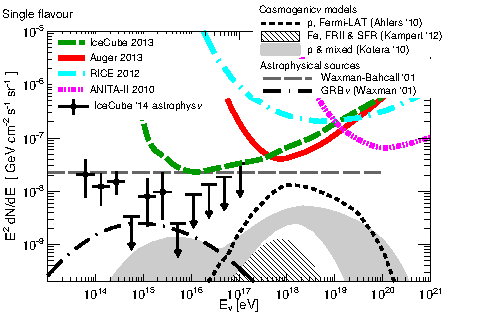
\includegraphics[width=0.75\textwidth]{fig/introduccion/1510-02050_multimessenger}
		\caption{\label{fig:multimess} Tomado de \cite{cite:multimess}. Flujo difuso de neutrinos medido por IceCube junto a los l\'imites impuestos por Auger, IceCube, Anita-II y Rice. Tambi\'en se muestran los flujos esperados para varios modelos cosmog\'enicos as\'i como la cota de Waxman-Bachall.}
		\end{center}
	\end{figure}
	
	Tanto IceCube como Auger han alcanzado exposiciones sin precedentes, lo que ha permitido descartar los modelos de AGN y los cosmog\'enicos m\'as optimistas, mientras que el resto de los que suponen protones como primario comienzan a verse desfavorecidos.
	Por otro lado, los que utilizan una componente primaria m\'as pesada se encuentran todav\'ia lejos del alcance de la detecci\'on actual.
	Por \'ultimo, una extrapolaci\'on del mejor ajuste del flujo medido por IceCube al rango de observaci\'on de Auger predice 0.1 eventos en su \'ultimo per\'iodo de medici\'on, compatible con una observaci\'on de 0 candidatos.
	
	Queda claro entonces que la nueva generaci\'on de detectores de neutrinos tiene mucho por descubrir.
	La observaci\'on del corte GZK respalda la existencia de un flujo cosmog\'enicos pero resultados recientes de Auger indican una migraci\'on hacia una componente m\'as pesada en los eventos de alta energ\'ia, lo que implicar\'ia flujos de neutrinos m\'as peque\~nos.
	Por este motivo la llegada de ARA, ARIANNA y GRAND generan mucha espectativa dentro de la comunidad.
	
% 	Esta tesis se encuentra dedicada al estudio de la detecci\'on de neutrinos c\'osmicos con detectores de superficie. 
% 	En la primer parte se presenta la b\'usqueda de neutrinos c\'osmicos realizada con el Observatorio Pierre Auger entre enero de 2004 y junio de 2013.
% 	Se describir\'a en detalle cada uno de los an\'alisis, los m\'etodos empleados en la discriminaci\'on de eventos candidatos y el c\'alculo de la exposici\'on, presentando por primera vez un resultado combinado, que dio lugar al l\'imite m\'as estricto publicado por Auger hasta la fecha.
% 	En la segunda parte se estudian las capacidades y limitaciones de un arreglo de antenas de radio al detectar neutrinos ultra energ\'eticos.
% 	Mediante simulaciones Monte Carlo se analiz\'o la factibilidad de la detecci\'on y se calcul\'o la exposici\'on que podr\'ia alcanzar un detector de las caracter\'isticas de GRAND.
% 	
	